\documentclass[11pt,a4paper]{article}
\usepackage{TeX_definitions}
\geometry{left=2.4cm,right=2.4cm,top=2.4cm,bottom=2.4cm}
\graphicspath{{figures/}}
\hypersetup{colorlinks=true,linkcolor=blue,citecolor=blue,urlcolor=blue}

\title{Analysis 4-6: standardising KL-based visual diagnostics}
\author{}
\date{\today}
\begin{document}
\maketitle

\section{Question}
Analysis 4-6 turns the family-separation workflow into a reusable visual standard. The aim is not new scientific inference, but reproducible and comparable reporting across future analyses.

\section{Method}
Standard graphical-model background and notation are treated in the usual way; see \cite{Koller2009}.


We audited the outputs generated in Analyses 4-2 and 4-3 and distilled them into a compact figure specification. The standard records figure types, mandatory status, required annotations, default metrics, filename rules, and a worked example panel.

\section{Results}
The mandatory default suite contains four figure types: \texttt{condition\_specific\_family\_divergence\_heatmap}, \texttt{target\_belief\_profile\_panel}, \texttt{global\_family\_confusion\_summary}, and \texttt{rooted\_descriptor\_linkage\_summary}. The worked example uses RG112 at high evidence and shows the recommended panel stack: graph/evidence visualisation, family divergence heatmap, and belief profile bars.

\begin{figure}[H]
\centering
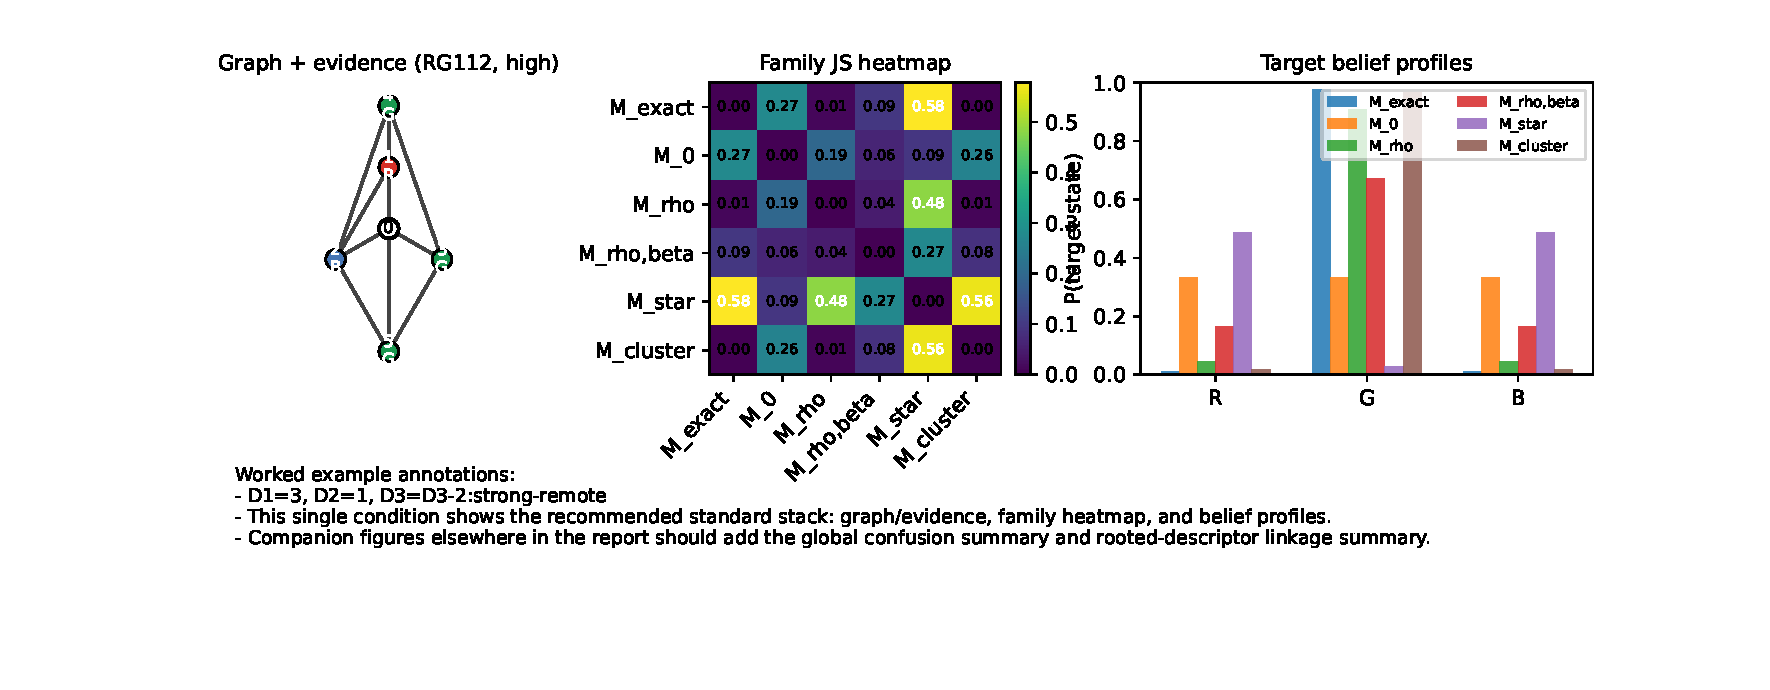
\includegraphics[width=\textwidth]{analysis-4-6_fig1_worked_example_panel.pdf}
\caption{Worked example of the standard condition-specific visual report.}
\end{figure}

\section{Conclusions against the TODO}
\begin{enumerate}
    \item Future diagnostics now have a compact default figure suite.
    \item The standard ties every figure type to a specific scientific question.
    \item D1/D2/D3 terminology is preserved from Analysis 3.
    \item The worked example is sufficient for collaborators and students to reproduce the intended style.
\end{enumerate}

\bibliographystyle{apalike}
\bibliography{../../manuscript/library}
\end{document}
